\renewcommand{\labelenumii}{\theenumii}
\renewcommand{\theenumii}{\theenumi.\arabic{enumii}.}

\section{User Documentation}
Test and manage your Web Applications security with a few clicks, The WASS software allows you to scan a Web Application for security vulnerabilities, save the results of the scan and generate reports in PDF, XML and TXT formats. 

\begin{enumerate}
    \item Create Account
    \begin{enumerate}
    
        \item The first step in order to use WASS is enter to              http://178.128.186.156:3000 in your favorite browser. 
        \begin{figure}[h!]
            \centering
            
\includegraphics[width=14cm]{img/userdoc1.png}
            \caption{WAAS URL}
            \label{fig:wass_url}
        \end{figure}
        
        \item  The next step is to create an user account, navigate to the software and you will see a login page
        \begin{figure}[h!]
            \centering
            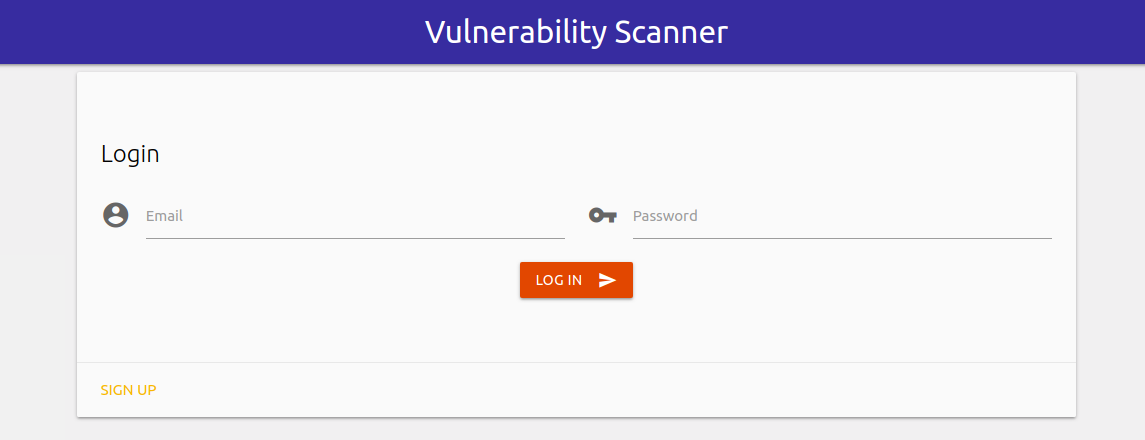
\includegraphics[width=12cm]{img/userdoc2.png}
            \caption{Login page}
            \label{fig:login_page}
        \end{figure}
        
        \item Click on sign up \\
        \begin{figure}[h!]
            \centering
            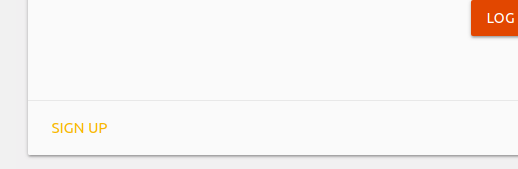
\includegraphics[width=14cm]{img/userdoc3.png}
            \caption{Sign up}
            \label{fig:sign_up}
        \end{figure}
        
        \item Insert your email, create a password and click on sign up.
        \begin{figure}[h!]
            \centering
            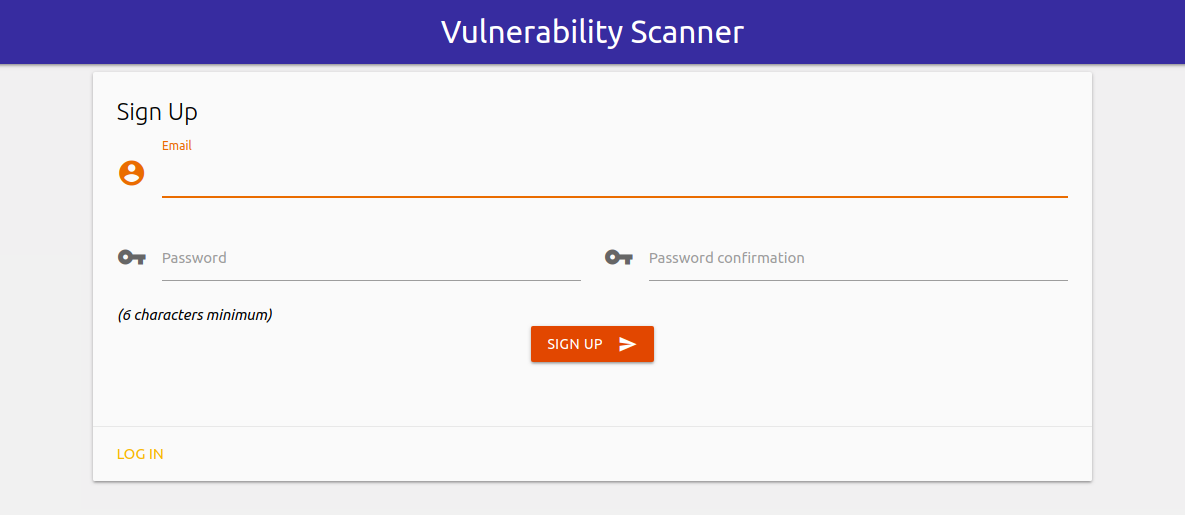
\includegraphics[width=14cm]{img/userdoc4.png}
            \caption{Sign up form}
            \label{fig:sign_up_form}
        \end{figure}
        
      \end{enumerate}
      
      \item Analysing a Web Application by URL 
      \begin{enumerate}
          \item Once you have your user account, login with your email and password and click on log in button.
          \begin{figure}[h!]
            \centering
            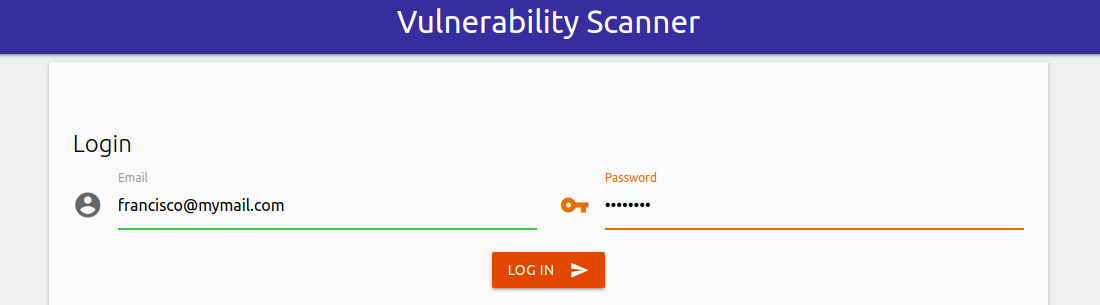
\includegraphics[width=12cm]{img/userdoc5.png}
            \caption{Log in form}
            \label{fig:log_in_form}
          \end{figure} 
          
           \item To analyze a web application, write or paste its URL into the URL field. If the web app you want to scan requires authentication provide the auth token.
           \begin{figure}[h!]
            \centering
            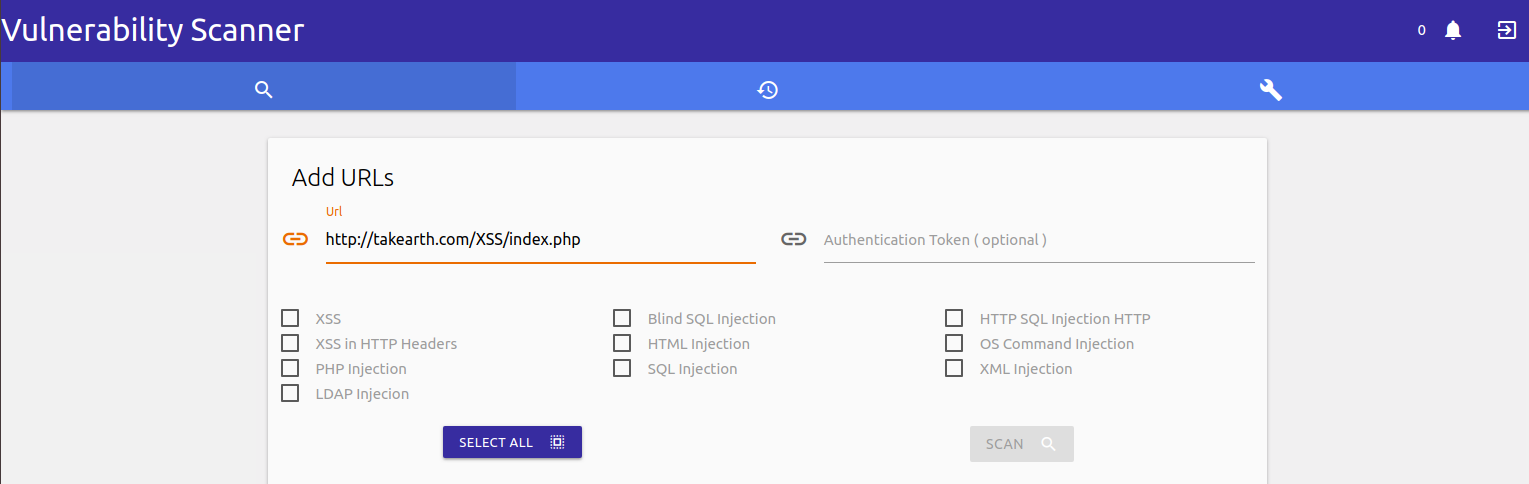
\includegraphics[width=14cm]{img/userdoc6.png}
            \caption{Scanner options}
            \label{fig:scanner_options}
          \end{figure} 
          
          \item Then select the vulnerabilities that you want to analyze and click SCAN \\
          \begin{figure}[h!]
            \centering
            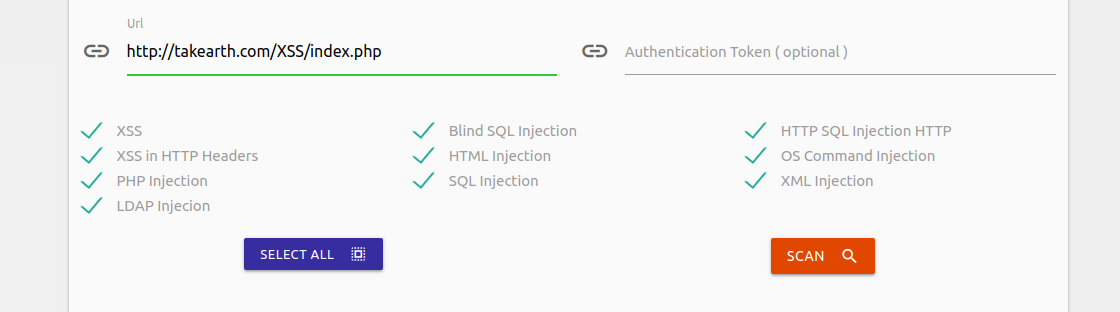
\includegraphics[width=14cm]{img/userdoc7.png}
            \caption{Vulnerabilities selected}
            \label{fig:vulnerabilities_selected}
          \end{figure} \\
          You can click on the select all button to enable all the possible scans\\
          
          \item You will be redirected to the dashboard
          \begin{figure}[h!]
            \centering
            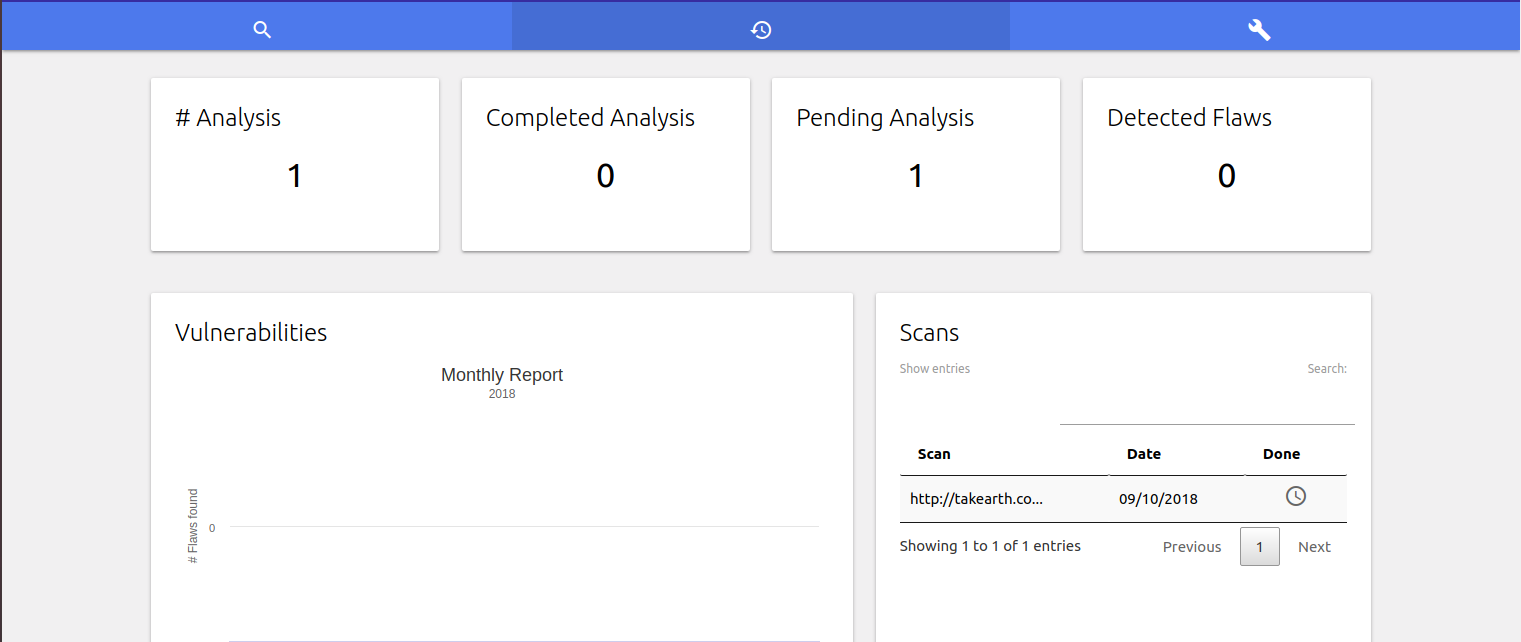
\includegraphics[width=12cm]{img/userdoc8.png}
            \caption{Dashboard}
            \label{fig:dashboard}
          \end{figure}
          
          
      \end{enumerate}
      
      \item Dashboard\\
      Here, you can see the information and results about previous scans.
      \begin{figure}[h!]
        \centering
        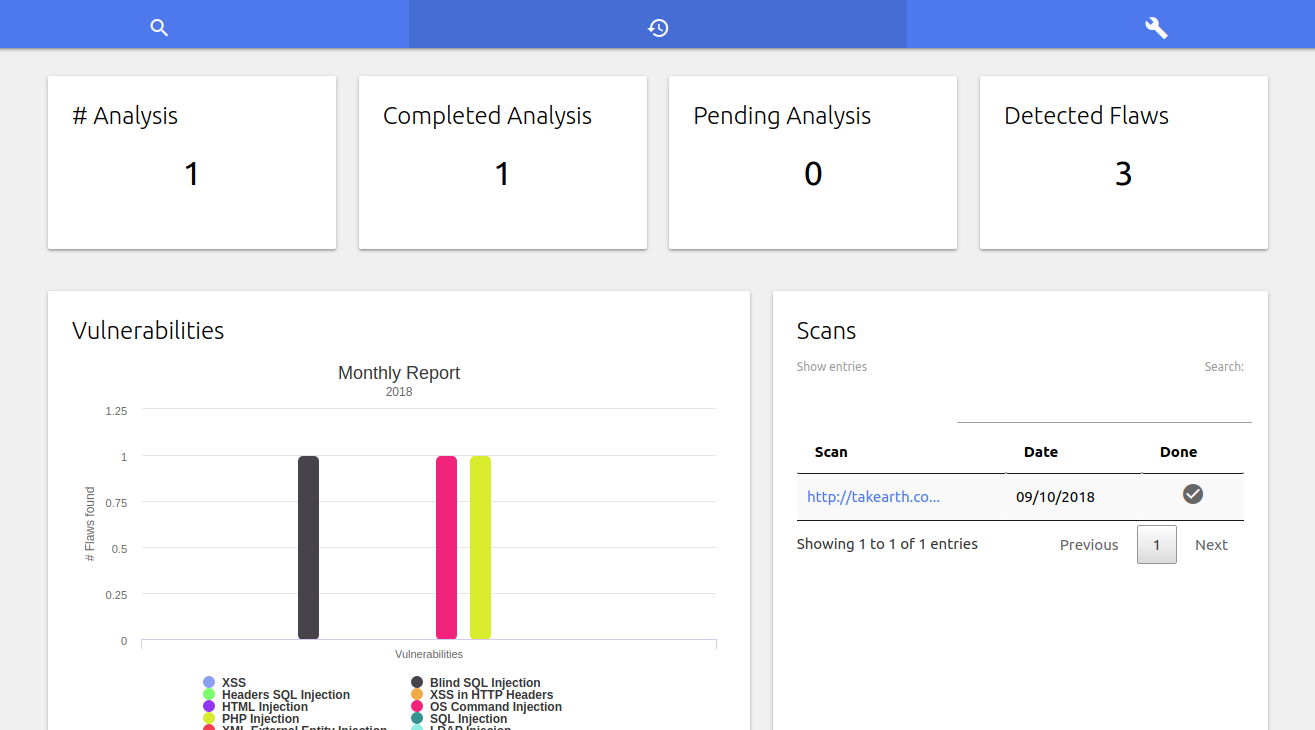
\includegraphics[width=14cm]{img/userdoc9.png}
        \caption{Dashboard}
        \label{fig:dashboard_graphics}
     \end{figure}
     \\
     In this page you can check the total number of analysis, the completed analysis, the pending analysis and the flaws detected.\\
     
     In the right top corner you can see the notifications and the logout buttons 
     \begin{figure}[h!]
        \centering
        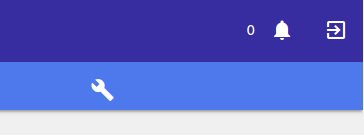
\includegraphics[width=14cm]{img/userdoc10.png}
        \caption{Notifications and log out options}
        \label{fig:notifications_logout}
     \end{figure}
     
     \clearpage
     You can see detailed information of any specific scan by clicking the url in the Recent Scans section \\
     \begin{figure}[h!]
        \centering
        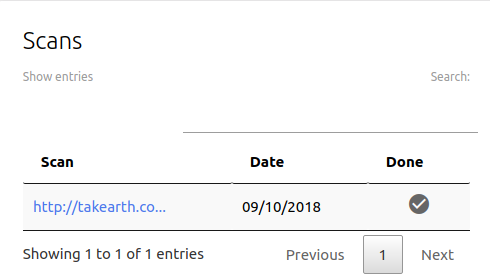
\includegraphics[width=14cm]{img/userdoc11.png}
        \caption{Recent Scans}
        \label{fig:recenly_scanns}
     \end{figure}
     \\
     Here you will see at the left the vulnerabilities found on the analyzed web page, on the right we see a detailed description of the vulnerability
     \begin{figure}[h!]
        \centering
        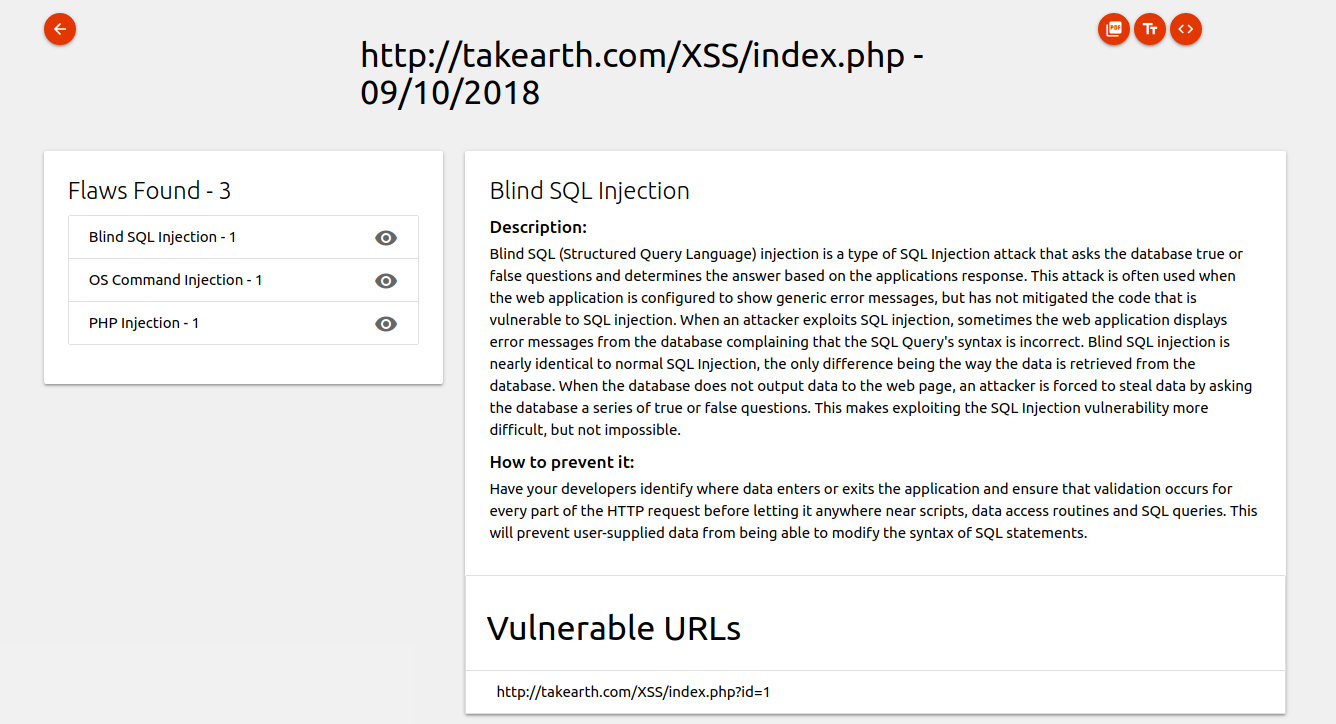
\includegraphics[width=14cm]{img/userdoc12.png}
        \caption{Vulnerabilities details}
        \label{fig:vulnerabilities_details}
     \end{figure}
     \\
     \clearpage
   The number at the right of the flaw represents the number of urls affected by this vulnerability inside the application
   \begin{figure}[h!]
        \centering
        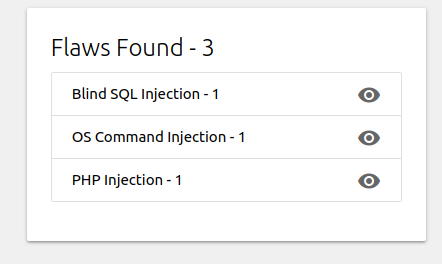
\includegraphics[width=14cm]{img/userdoc13.png}
        \caption{Flaws found}
        \label{fig:flaws_found}
   \end{figure}
   
   \item Exporting reports \\
   You are able to export this analysis in PDF, XML and in plain text or TXT, in order to do this click on the icons on the top right
   \begin{figure}[h!]
        \centering
        
\includegraphics[width=14cm]{img/userdoc14.png}
        \caption{Export icons}
        \label{fig:export_icons}
   \end{figure}
   \clearpage
   When you click on one of the icons a download will start  
   \begin{figure}[h!]
        \centering
        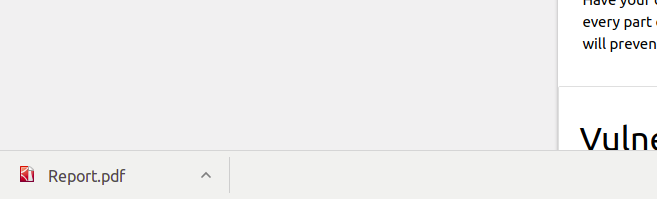
\includegraphics[width=14cm]{img/userdoc15.png}
        \caption{File Downloaded}
        \label{fig:file_downloaded}
   \end{figure}
   \\
   You should be able to open the file on your prefered reader.
   \begin{figure}[h!]
        \centering
        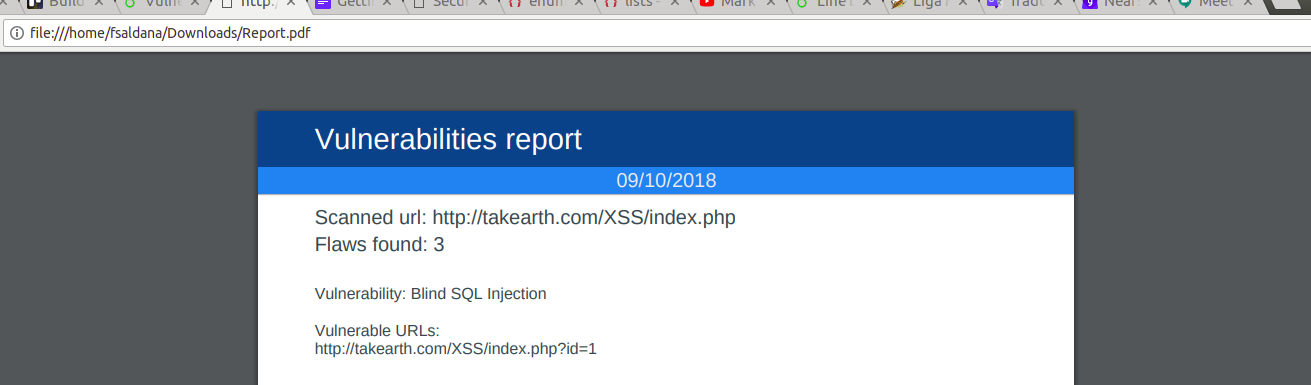
\includegraphics[width=14cm]{img/userdoc16.png}
        \caption{Report}
        \label{fig:report}
   \end{figure}
   
   \item Managing your account \\
   You are able to modify your account email and password, if you want to change one just go to the wrench icon, it's the menu at the right.
   \begin{figure}[h!]
        \centering
        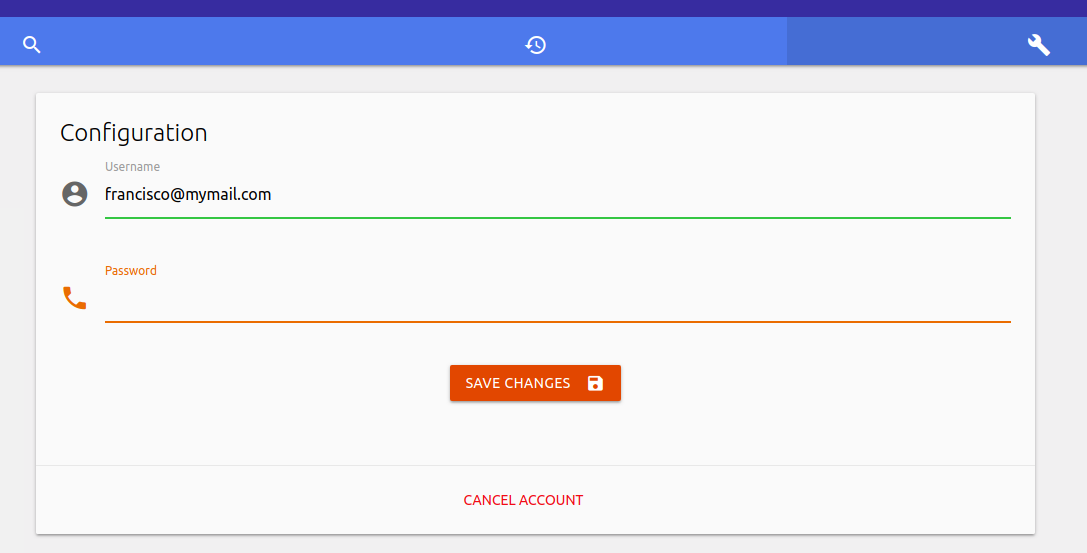
\includegraphics[width=12cm]{img/userdoc17.png}
        \caption{Account configuration}
        \label{fig:account_configuration}
   \end{figure}
   \\
   \\
   Update your credentials and click on SAVE CHANGES in order to conserve the changes, you will be asked to sign up again in order to continue using the scanner.
   \begin{figure}[h!]
        \centering
        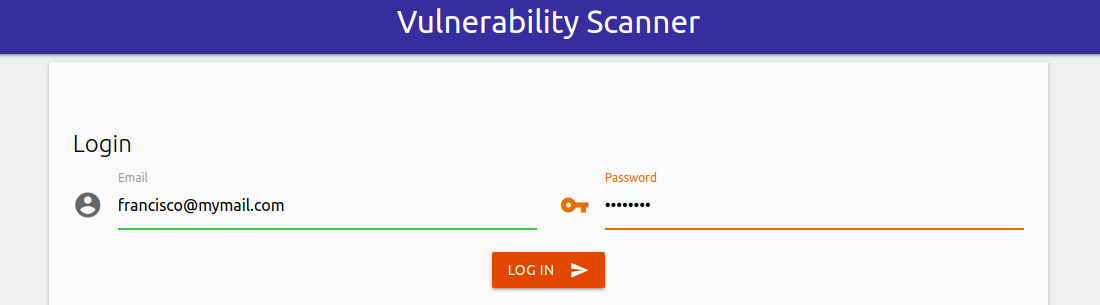
\includegraphics[width=12cm]{img/userdoc5.png}
        \caption{Log in}
        \label{fig:log_in}
   \end{figure}
   
   
   
\end{enumerate}



\clearpage